\begin{mainquestion}{rlrcstep}{Capacitor and Inductor Experiment}
Your lab partner was experimenting with the following circuit:

\begin{center}
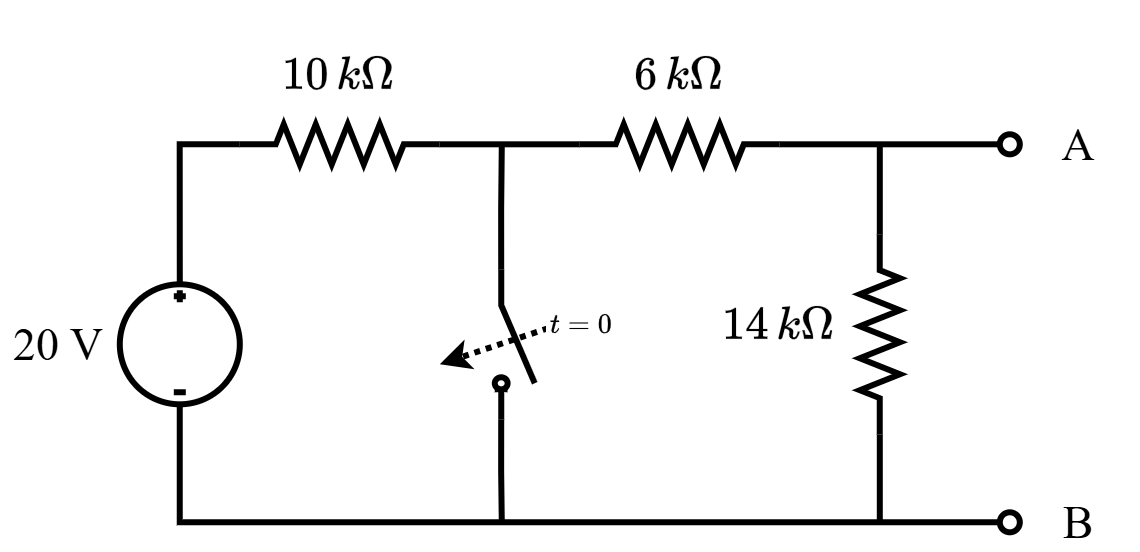
\includegraphics[width=0.8\textwidth]{figure1.png}
\end{center}
They connected a \SI{300}{\milli\henry} inductor between terminals A and B, and left it hooked up for quite some time.

\begin{partquestion}{current0}{What is the current through the inductor $i_L(0^-)$?}
\begin{answer}
At DC, the inductor acts like a short. It follows that
\begin{align*}
 i_L(0^-)
 &= \frac{\SI{20}{\volt}}{\SI{10}{\kilo\ohm}+\SI{6}{\kilo\ohm}} \\
 &= \SI{1.25}{\milli\ampere}.
\end{align*}
\end{answer}
\end{partquestion}
\begin{partquestion}{currentt}{Your partner wants to find the inductor's current behavior. If the switch is closed at time $t=0$ seconds, what is the current through the inductor $i_L(t)$ for time $t>0$?}
\begin{answer}
After the switch is closed, the circuit looks as follows:
\begin{center}
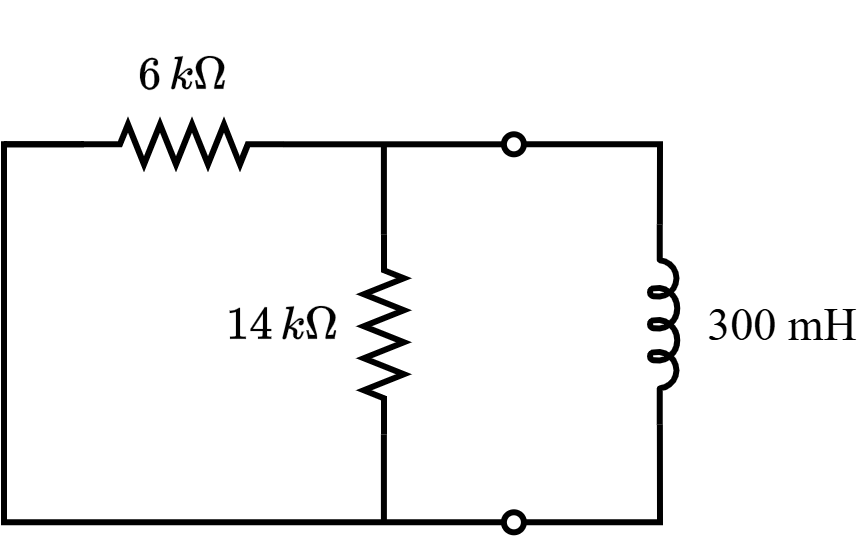
\includegraphics[width=0.8\textwidth]{figure2.png}
\end{center}
The current through the inductor will decay exponentially based on the time constant according to
\begin{equation*}
 i_L(t)=i_L(0^-)e^{-t/\tau_L},
\end{equation*}
where
\begin{align*}
 \tau_L
 &= \frac{L}{R_{\mathrm{eq}}} \\
 &= \frac{\SI{0.300}{\henry}}
 {\SI{6}{\kilo\ohm}\parallel\SI{14}{\kilo\ohm}} \\
 &= \frac{(\SI{0.300}{\henry})(\SI{20}{\kilo\ohm})}
 {\SI{84}{\kilo\ohm\squared}} \\
 &= \SI{7.14e-5}{\second}.
\end{align*}
This gives
\begin{equation*}
 \boxed{i_L(t)=(\SI{1.25}{\milli\ampere})e^{-t/(\SI{7.14e-5}{\second})}},
 \qquad t>0.
\end{equation*}


\end{answer}
\end{partquestion}
\begin{partquestion}{cap}{You find an unmarked capacitor on the bench. You remove the inductor, open the switch again, and place the mysterious capacitor between terminals A and B and leave it hooked up for quite some time. You measure the voltage across the capacitor $v_C(t)$ after you close the switch at the start of your analysis, which we can again call $t=0$. Incredibly, it is a scaled copy of your partner's graph of $i_L(t)$. What is the value $C$ of the capacitor?}
\begin{answer}
At DC, the capacitor acts like an open. It follows that
\begin{align*}
 v_C(0^-)
 &= \frac{\SI{14}{\kilo\ohm}}
 {\SI{10}{\kilo\ohm}+\SI{6}{\kilo\ohm}+\SI{14}{\kilo\ohm}}
 (\SI{20}{\volt}) \\
 &= \SI{9.33}{\volt}.
\end{align*}

After the switch is closed, the circuit looks as follows:
\begin{center}
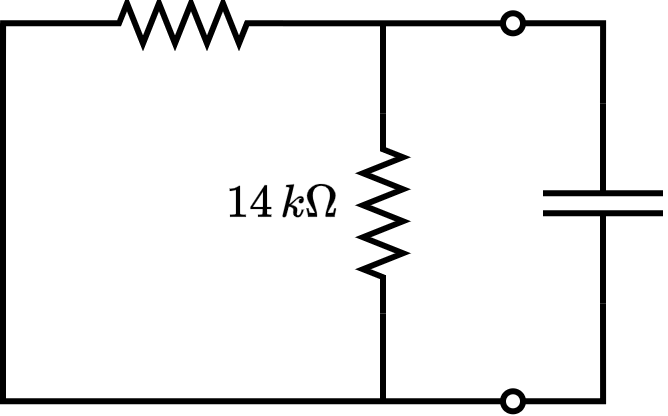
\includegraphics[width=0.8\textwidth]{figure3.png}
\end{center}
The voltage across the capacitor will decay exponentially based on the time constant according to
\begin{equation*}
 v_C(t)=v_C(0^-)e^{-t/\tau_C},
\end{equation*}
where
\begin{equation*}
 \tau_C=R_{\mathrm{eq}}C
 =\left(\SI{6}{\kilo\ohm}\parallel\SI{14}{\kilo\ohm}\right)C.
\end{equation*}
For this to have the exact same shape, the exponential terms must be identical, which means that the time constants are also equal:
\begin{equation*}
 \tau_L=\tau_C.
\end{equation*}
This implies
\begin{align*}
 \left(\SI{6}{\kilo\ohm}\parallel\SI{14}{\kilo\ohm}\right)C
 &= \SI{7.14e-5}{\second}, \\
 C
 &= \frac{\SI{7.14e-5}{\second}}{\SI{4200}{\ohm}} \\
 &\approx \boxed{\SI{17}{\nano\farad}}.
\end{align*}

Did you see that coming?
\end{answer}
\end{partquestion}
\begin{partquestion}{ratio}{What is the ratio $v_C(t)/i_L(t)$ (with units)? What is the significance of this ratio? }
\begin{answer}
Because the two waveforms have identical exponential factors,
\begin{align*}
 \frac{v_C(t)}{i_L(t)}
 &= \frac{v_C(0^-)}{i_L(0^-)} \\
 &= \frac{\SI{9.33}{\volt}}{\SI{1.25}{\milli\ampere}} \\
 &= \boxed{\SI{7.47}{\kilo\ohm}}.
\end{align*}
This ratio is just the Th\'evenin resistance as seen by the load before the switch is thrown.
\end{answer}
\end{partquestion}
\begin{partquestion}{energy}{Find the approximate energy lost by your lab partner's inductor \SI{500}{\micro\second} after the switch was closed in part (\cref{prob:rlrcstep:currentt}). Find the approximate energy lost by your capacitor \SI{500}{\micro\second} after the switch was closed in part (\cref{prob:rlrcstep:cap}). In both cases, state where this energy went.}
\begin{answer}
\SI{500}{\micro\second} is more than five time constants, so we can assume that the inductor current and capacitor voltage have both reached zero by that time, and that each has lost all the energy it originally had when the switch was thrown.

For the inductor,
\begin{align*}
 E_L
 &= \frac{1}{2}L\left[i_L(0^-)\right]^2 \\
 &= \frac{1}{2}(\SI{0.300}{\henry})
    (\SI{0.00125}{\ampere})^2 \\
 &= \boxed{\SI{234}{\nano\joule}}.
\end{align*}

For the capacitor,
\begin{align*}
 E_C
 &= \frac{1}{2}C\left[v_C(0^-)\right]^2 \\
 &= \frac{1}{2}(\SI{17e-9}{\farad})(\SI{9.33}{\volt})^2 \\
 &\approx \boxed{\SI{740}{\nano\joule}}.
\end{align*}

In both cases, all the energy was absorbed in the \SI{6}{\kilo\ohm} and \SI{14}{\kilo\ohm} resistors and converted to heat.
\end{answer}
\end{partquestion}
\begin{partquestion}{charge}{Find the total charge that flows through the inductor in the first \SI{170}{\micro\second} after the switch closes in part (\cref{prob:rlrcstep:currentt}).}
\begin{answer}
\begin{align*}
 Q
 &= \int_0^{\SI{170}{\micro\second}} i_L(t)\,dt \\
 &= \int_0^{\SI{170}{\micro\second}}
 (\SI{0.00125}{\ampere})e^{-t/(\SI{7.14e-5}{\second})}\,dt \\
 &= -\left(\SI{7.14e-5}{\second}\right)
    (\SI{0.00125}{\ampere})
    e^{-t/(\SI{7.14e-5}{\second})}
    \bigg|_0^{\SI{170}{\micro\second}} \\
 &\approx \SI{8.1e-8}{\coulomb} \\
 &= \boxed{\SI{81}{\nano\coulomb}}.
\end{align*}
\end{answer}
\end{partquestion}
\end{mainquestion}